\documentclass[10pt,journal,compsoc]{IEEEtran}



% *** CITATION PACKAGES ***
%
\ifCLASSOPTIONcompsoc
  % The IEEE Computer Society needs nocompress option
  % requires cite.sty v4.0 or later (November 2003)
  \usepackage[nocompress]{cite}
\else
  % normal IEEE
  \usepackage{cite}
\fi

% *** GRAPHICS RELATED PACKAGES ***
%
\ifCLASSINFOpdf
 
\else
  
\fi


\usepackage{graphicx}

\newcommand\MYhyperrefoptions{bookmarks=true,bookmarksnumbered=true,
pdfpagemode={UseOutlines},plainpages=false,pdfpagelabels=true,
colorlinks=true,linkcolor={black},citecolor={black},urlcolor={black},
pdftitle={Bare Demo of IEEEtran.cls for Computer Society Journals},%<!CHANGE!
pdfsubject={Typesetting},%<!CHANGE!
pdfauthor={Michael D. Shell},%<!CHANGE!
pdfkeywords={Computer Society, IEEEtran, journal, LaTeX, paper,
             template}}%<^!CHANGE!

\hyphenation{op-tical net-works semi-conduc-tor}

\begin{document}

\title{QoS-Oriented Mobile Service Composition Over Oppotunistic Networks}

\author{Qinglan~Peng,~\IEEEmembership{Member,~IEEE,}
        John~Doe,~\IEEEmembership{Fellow,~OSA,}
        and~Jane~Doe,~\IEEEmembership{Life~Fellow,~IEEE}% <-this % stops a space
\IEEEcompsocitemizethanks{\IEEEcompsocthanksitem M. Shell was with the Department
of Electrical and Computer Engineering, Georgia Institute of Technology, Atlanta,
GA, 30332.\protect\\
% note need leading \protect in front of \\ to get a newline within \thanks as
% \\ is fragile and will error, could use \hfil\break instead.
E-mail: see http://www.michaelshell.org/contact.html
\IEEEcompsocthanksitem J. Doe and J. Doe are with Anonymous University.}% <-this % stops a space
\thanks{Manuscript received April 19, 2005; revised August 26, 2015.}}



% The paper headers
\markboth{Journal of \LaTeX\ Class Files,~Vol.~14, No.~8, August~2015}%
{Shell \MakeLowercase{\textit{et al.}}: Bare Advanced Demo of IEEEtran.cls for IEEE Computer Society Journals}

\IEEEtitleabstractindextext{%
\begin{abstract}
The abstract goes here.
\end{abstract}

% Note that keywords are not normally used for peerreview papers.
\begin{IEEEkeywords}
Computer Society, IEEE, IEEEtran, journal, \LaTeX, paper, template.
\end{IEEEkeywords}}


% make the title area
\maketitle



\IEEEdisplaynontitleabstractindextext

\IEEEpeerreviewmaketitle


\ifCLASSOPTIONcompsoc
\IEEEraisesectionheading{\section{Introduction}\label{sec:introduction}}
\else
\section{Introduction}
\label{sec:introduction}
\fi


\IEEEPARstart{R}{ecent years}, with the rapid developments of mobile devices and wireless communication technologies, web services are no longer limited to traditional platforms and they are becoming more flexible and pervasive \cite{Deng2017}. The hardware of mobile devices will continue make breakthroughs to extend mobile devices’ capabilities in terms of memory, computational power, storage capacity, and so on \cite{Deng2017}. Mobile technology’s huge potential brings great opportunities to traditional service computing in the mobile environment \cite{Deng2016}, As a result, the global interest of mobile applications is on the rise. Both researchers and industrial companies are inspired to pave the road for mobile Web service provisioning \cite{dinh2013survey,hu2014multidimensional}\cite{Deng2017}.

While mobile device have powerful computing and communication capabilities, the high data rate services, however, drain out the energy of the device much faster than before **[Call for Papers]**. 

To achieve the goal of reducing mobile device energy consumption, in this paper we advocate a QoS-oriented mobile service composition over opportunistic approach, where a mobile user in opportunistic can combine and exploit each other’s resources to boost their computing power and overcome the limitations of their own resources without the communication energy footprint and the extreme centralization of mobile cloud computing (As shown in fig.1) \cite{Giordano2011}. Its main rationality is three-fold. First, opportunistic user encounters are prevalent and sufficient in daily life \cite{liu2013exploring}, which offers plenty of opportunities to exploit nearby mobile worker for task solving [T], [T], [T]. Second, many mobile tasks require huge computational resources or data trasfer  (e.g., Tensorflow on mobile, Photoshop on mobile, Online video), for an energy consumption and cost perspective, nearby mobile service provider are more adept at executing them than the online workers, because this paradigm can reduce data transfer over cellular network which consume more energy than device to device (D2D) communications such as Bluetooth, NFC, WiFi-direct and LTE-D2D \cite{}\cite{}. Third, D2D communications are promising to replenish traditional cellular communications in terms of user throughput increase, cellular traffic reduction and network coverage extension,  in this way, users can get better quality of service and save communication fee at the same time \cite{asadi2014survey}. In a word, this framework shares the similar spirit with the emerging paradigm “cyber foraging” over opportunistic networks, such that mobile users opportunistically exploit nearby device resources to facilitate their computational task processing \cite{shi2012serendipity,li2014can,zhang2015offloading}\cite{Pu2017}.

\begin{figure}[!t]
\centering
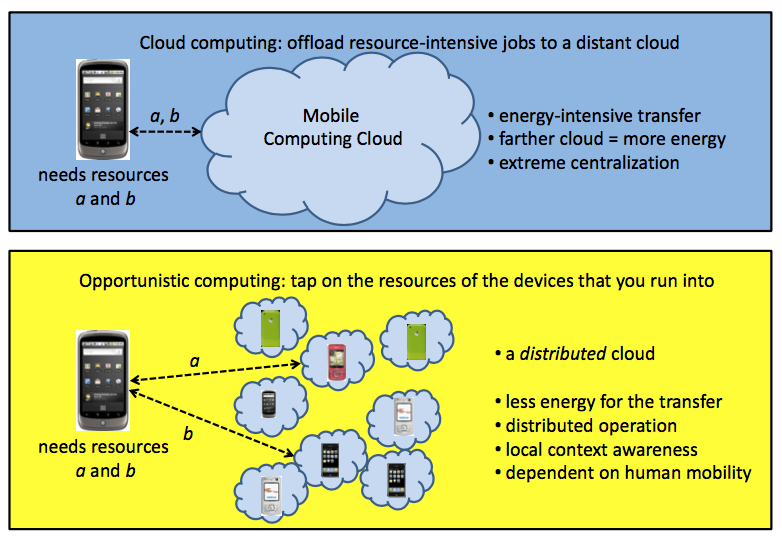
\includegraphics[width=2.5in]{./img/fig1.png}
\caption{SensorDistance.}
\label{fig_sim}
\end{figure}

To address the aforementioned challenges and concerns, we propose a new approach for service selections and compositions in mobile opportunistic network. The main contributions are:

1) We propose an framework for mobile service provision [mobile service opportunistic network MSON] to address the problem of service selection for mobile service composition in the mobile encounter enviroment where both service requesters and providers are nonstationary. In such environment, mobile user can share mobile services with nearby mobile devices through D2D links.

2) For MSON, we propose a mobile service QoS model for service provision which consider mobile service availability as an important QoS attribute to capture user's mobility behavior.

3) Based on MSON and the proposed mobile service QoS model, we transfer the mobile service composition over opportunistic problem to an optimization problem and propose to utilize the Krill-Herd algorithm (KH) to solve it. We conduct aseries of evaluations to validate that our algorithmis approximately optimal and performs much better than other standard composition approaches. We compare it with other population-based optimization methods for both optimality and scalability. 

The remainder of this paper is organized as follows. Section II describe the MSON framework and its application scenario. Section III introduces the mobile service composition model. The approach to make service compositions is presented in Section IV. Section V presents experimental results. Section VI reviews the related work. Section VI concludes this paper.

\section{MSON AND APPLICATION SCENARIO}

\begin{figure}[!t]
\centering
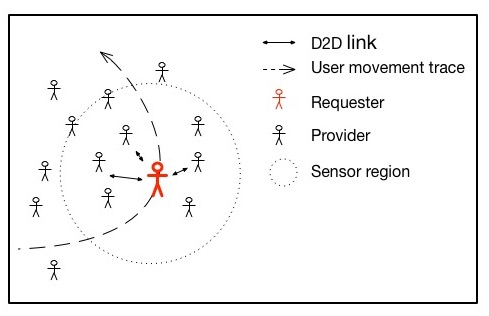
\includegraphics[width=2.5in]{./img/fig2.jpg}
\caption{SensorDistance.}
\label{fig_sim}
\end{figure}

In this section, we introduce the mobile service opportunistic network (MSON) formed by multiple mobile users. Within it, users can share services on their own mobile devices through opportunistic mobile networks. Its three main characteristics as follows \cite{Deng2017}.

1) Locality: An MSON is not established on the Internet, it do not consider user mobility a problem but as an opportunity to exploit. Mobile user in opportunistic network can sense each other's service and establish self-orginzed local communication network within sensor distance.

2) Dynamicity: MSON participants are not stationary. They can enter or leave the self-orginzed group at any time.

3) Mobility: Services provided by mobile users are not fixed at the same location. Service requesters are also mobile when invoking a mobile service.

Fig.2 illustrates the working procedure of the mobile service provision over opportunistic network. In an opportunistic network scenario, a mobile task requester $R$ can sense mobile service exposed by nearby devices through D2D link and launches a mobile composotion request. 

A composer can be implemented and deployed on the requester’s mobile device, which is in charge of discovering available mobile services nearby, composing multiple services, and selecting appropriate service candidates for composition tasks. Note that the service candidates are selected for all the tasks before the execution of the composition. During the execution of mobile service compositions, all the component services interact with the composer directly. The communication among mobile devices is based on Bluetooth, WLAN, or other available D2D communication protocols \cite{Deng2017}.

We should emphasize that, our framework only considers one-hop mechanism for both service provider and consumer, since realistic dataset analyses reveal that users’ one-hop neighbors are sufficient \cite{liu2013exploring} and can cover most range of the whole network in a reasonable time period \cite{fan2011delque}, and contacting a user would incur long delay if the maximum D2D communication hops are larger than two \cite{li2014can}. Compared with multi-hop mechanisms in existing researches \cite{chang2015progressive,karaliopoulos2015user,han2016competition,tuncay2013participant,wu2013homing,jiang2016exploiting}[1], this one-hop feature can lower the network overhead (e.g., no need to transfer a large volume of task contents hop by hop) and ensure framework performance with only local information, which is more practical in real life \cite{Pu2017}. Hence, once two mobile devices are out of their sensing distance, they would lose the connection \cite{Deng2017}. 

we use an example depicted in Fig.1 to illustrate the related features of the problem of MSON. Assume mobile user Mike just complete his tour and now he is on the subway to airport. Now he wants to edit the video he recorded and add some effects and share the video clip to his friends. But due to mobile devices' limited battery, if he invoke clip service in his own device, his mobile phone will shutdown before he reach the destination because of run out of energy. As one option, he can upload the video to cloud services to get the video clip, but offloading quest into cloud will result in heavy cellular traffic, that means expensive communication fee and high energy consumption \cite{,,}. If Mike participate in MSON and servel video processing services is provided by some nearby mobile devices, Mike can invoke such mobile services on nearby mobile devices through free near field communication techniques. If these services cannot meet his requirement, several services can be composed. For example in Fig. 2, at most three services are needed: 1) video cutting service; 2) video beautifying service; and 3) video share service. Due to users’ mobility, the availability of service to Mike can vary, we will discuss mobile service availability in next section. In this environment invoking services provided by other mobile users may face new challenges that traditional composition methods cannot handle, thus, a mobile service composition model which can capture mobile services' availability need to be proposed \cite{Deng2016-2}.


\section{MOBILE SERVICE COMPOSITION MODEL}
In this section, we first give some basic definition of mobile web service, then introduce the concept of mobile service availability, and propose specific QoS model for mobile service composition over opportunistic network \cite{Deng2016-2}.
\subsection{Preliminaries}
In order to describe the problem addressed in this paper, we first provide the basic concepts of mobile service composition based on the proposed mobility model.

\textit{Definition 1 (Mobile Service):} A mobile service is a triple $s = (uuid, Fun, QoS)$, where:

​	1) $uuid$ is the unique identifier of the service;

​	2) $Fun$ is the set of functions s provides, a function includes the input, output, precondition and result of the service;

​	3) $QoS = \{q\}^n_{j=1}$ is a set of quality attributes, including execution cost, response time, reliability, availability, etc \cite{Deng2016-2}.

\textit{Definition 2 (MSON participant):} A MSON participant is mobile service user who can be both service provider and consumer, it can be represented by three-tuple $u = (uuid, P, C)$, where:

​	1) $uuid$ is the unique identifier of the provider;

​	2) $P$ is the set of mobile services exposed by mobile service user $u$.

​	3) $C$ is the set of perceived mobile services from nearby mobile service users.

\textit{Definition 3 (Mobile Service Composition Plan):} A service composition plan is a tuple $scp = (T, R)$, where:

​	1) $T = \{t_1,t_2,…,t_n\}$ is a set of tasks;

​	2) $R = \{d(t_i,t_j)|t_i,t_j \in T\}$ is a set of relations between tasks in $L$.

​	A service composition plan is an abstract description of a business process. Each task $l_i$ can be realized by invoking an individual service. There may be multiple services with different QoS that can be adopted to fulfill each task. $R$ is used to describe the structure of the composition. $d(t_i, t_j) = 1$ represents that the inputs of $t_j$ depend on the outputs of $t_i$ \cite{Deng2016-2}.

\textit{Definition 4 (composite service instance):} A service composition instance is a tuple $csi = (scp, S)$, where:
​	1) $scp$ is mobile service composition plan whitch defined in definition 3;

​	2) $S = {s_1, s_2,…,s_n}$ is a set of selected concrete tasks.

\subsection{Concept of Mobile Service Availability}
In mobile service opportunistic network (MSON) the availability of service to its invoker is highly related to the user’s mobility. If user $i$ moves outside the transmission range of its neighbouring user $j$, then user $i$ is unreachable by user $j$ and as a result the services on user $i$ become unavailable to user $j$ either. Here user mobility is utilized to calculate the mobile service availability \cite{Yang2010}.

\textit{Definition 5 (Mobile Service Availability):} mobile service availability can be represented by a 3 tuple $(I, P, V) $, where

​	1) $I$ is the mobile service consumer;

​	2) $P$ is the mobile service provider;

​	3) $V$ is the mobile service availability value between consumer and provider, $V \in [0,1)$, and $V=0$ means service provider moves out of service sensor range.


\begin{figure}[!t]
\centering
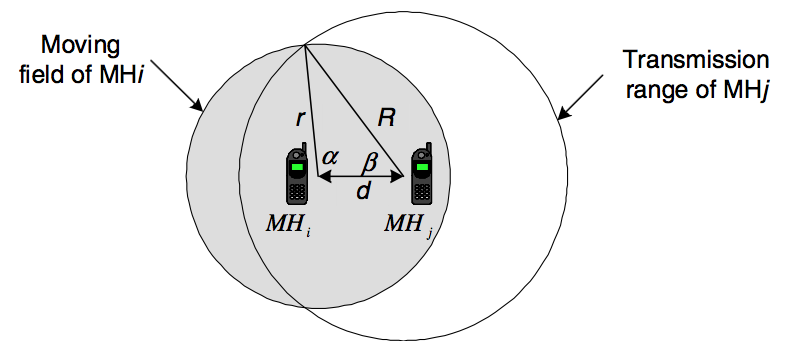
\includegraphics[width=2.5in]{./img/fig3.png}
\caption{SensorDistance.}
\label{fig_sim}
\end{figure}

As illustrated in Fig. 2, consider two mobile users $MU_i$ and $MU_j$ of the same transmission range $R$. Each node moves randomly and it is assumed that the moving field is a circle with a radius of $r$. $d$ represents the distance between $MU_i$ and $MU_j$. These three parameters are to be used for calculating the node availability. The transmission range of a node $R$ is known (e.g., pre-defined or changing according to certain algorithm). Suppose the location (i.e., coordinates) of each mobile host is known (e.g., via GPS—global positioning system, **How to get user's moving trace, refer S.Deng's work **), then distance $d$ can be calculated using the Euclidean distance formula, i.e.,$\sqrt{{(x_i-x_j)^2}+{y_i-y_j}^2}$ where $(x_i, x_j)$ and $(y_i, y_j)$ are are the coordinates of $MU_i$ and $MU_j$ respectively. Finally let us discuss how to calculate $r$ \cite{Yang2010}.


The moving radius of a mobile user $r$ is its speed $s$ multiplied by the average service time $t$. Here $t$ can be statistically calculated as the average value of last $n$ servings of this component service, namely, $t = \Sigma_{i=1}^{n}t_i/n$. The speed of a mobile host $s$ can be calculated based on its moving distance during a period from $t_1$ to $t_2$ \cite{ko2000location}, namely: $s = \sqrt{{(x_i-x_j)^2}+{y_i-y_j}^2}/(t_2-t_1)$. Then $r = s \times t$ \cite{Yang2010}.

​	Knowing the values of these three parameters $R$, $r$, and $d$, the probability of $MU_i$ staying inside the transmission range of $MU_j$ (denoted as $P_i^{IN}$ ) can be calculated by

\begin{equation}
P_i^{IN} = \frac{S_i^{IN}}{S_i^T}
\end{equation}

Namely, $P^{IN}_i$ equals to the area of the $MH_i$’s moving field inside the transmission range of $MU_j$ (denoted as $S^{IN}_i$) divided by the overall area of the $MU_i$’s moving field ($S^T_i$) \cite{Yang2010}.

\begin{eqnarray}
\alpha = arcons(\frac{r^2+d^2-R^2}{2r\times d}) \\
\beta = arcons(\frac{R^2+d^2-r^2}{2r\times d})
\end{eqnarray}

Then,

\begin{eqnarray}
S^{IN}_i = [(\frac{2\beta}{2\pi}\pi R^2)-(\frac{R sin\beta cos\beta}{2}2)]\\\nonumber
+ [(\frac{2\alpha}{2\pi}\pi r^2)-(\frac{r sin\alpha cos\alpha}{2}2)]\\\nonumber
= \beta R^2 + \alpha r^2 - (R^2 sin\beta cos\beta + r^2 sin\alpha cos\alpha)
\end{eqnarray}

There is also

\begin{equation}
S_i^T = \pi r^2 = \pi \times (s \times t)^2
\end{equation}

Therefore, we obtain

\begin{equation}
P_i^{IN} = \frac{S_i^{IN}}{\pi s^2 t^2}
\end{equation}

The probability of $MU_i$ staying inside the transmission range of $MU_j (P^{IN}_i)$ can be calculated. Suppose service $s$ running on $MU_i$ is a candidate service for a task running on $MH_j$, and the node availability with regard to concrete service $s$ is denoted as $q_{ava}(s)$, then finally there is

\begin{eqnarray}
q_{ava}(s) = P^{IN}_i = \frac{A_i^{IN}}{\pi s^2 t^2}\\\nonumber
= \frac{\beta R^2 + \alpha r^2 - (R^2 sin\beta cos\beta + r^2 sin\alpha cos\alpha)}{\pi s^2 t^2}
\end{eqnarray}

Note that, mobile service availability $q_{ava}(s)$ is an important QoS attribute to construct QoS model over MSON for service selection in next section.


\subsection{QoS Model for Mobile Service Composition}

For mobile service consumer to select concrete service, they must consider QoS \cite{wu2013predicting,luo2014efficient,luo2016generating}. Common QoS attributes include response time, price, reliability, and reputation, mobile service availability is an important QoS attribute introduced in this paper to describe user's mobility behavior. for mobile service composition in this paper. and they can be classified into two categories: 1) positive and 2) negative (denoted as $Q^+$ and $Q^−$). For positive attributes, larger values indicate better performance (e.g., repution and availability), while for negative attributes, smaller values indicate better performance (e.g., price and response time) \cite{Wu2016}.	

\begin{figure}[!t]
\centering
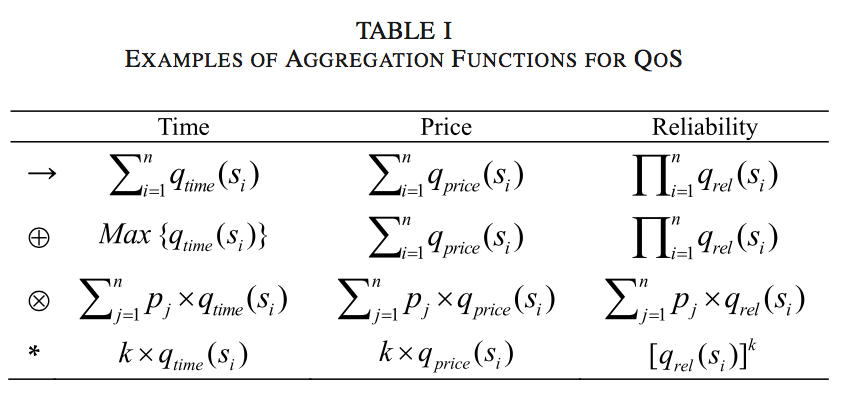
\includegraphics[width=2.5in]{./img/fig4.png}
\caption{SensorDistance.}
\label{fig_sim}
\end{figure}

For a composite service instance $csi$, the value of each QoS attribute is determined by the QoS values of its concrete components and orchestration patterns. Table $I$ lists the aggregation functions for response time, price, and availability for sequential, parallel, choice, and loop composition patterns, where $p_j$ represents the execution probability of the $j$th branch statement in the choice structure, and $k$ is the expected number of iterations of the loop. More aggregation functions can be found in \cite{jaeger2004qos} and \cite{zheng2013qos}.

In order to facilitate ranking of different composite service instances in terms of QoS, simple additive weighting (SAW) is used as the QoS utility function to map the QoS vector into a real value. SAW first normalizes the QoS attribute values into real values between $0$ and $1$, through comparison with the maximal and minimal values; then it sums the normalized values multiplied with a preference weight $w_t$. According to SAW, the QoS utility of a composite service instance $csi$ can be calculated using (1), where, $q_t(csi)$ is the aggregated value of the $t$-th QoS attribute of $csi$, and $q_{t,max}$ and $q_{t,min}$, respectively, denote the maximal and minimal possible aggregated values of the $t$th QoS attribute \cite{Wu2016}.

\begin{eqnarray}
U(csi) = \sum_{q_t \in Q^-} \frac{q_{t,max}-q_t(csi)}{q_{t,max}-q_{t,min}}\times w_t \\\nonumber
+\sum_{q_t \in Q^+} \frac{q_t(csi)-q_{t,max}}{q_{t,max}-q_{t,min}}\times w_t
\end{eqnarray}

\subsection{Problem Formulation}
Base on the above discussion, we can give the definition of the MSON service composition problem.

\textit{Definition 6 (MSON Service Composition):} Given a service composition request $req$ by a mobile user $u$, sense and select suitable concrete services provided by near mobile service provider to achieve an optimal service composition instance $csi$ with the best QoS value. Meanwhile, $csi$  should be the optimal in terms of QoS utility and also satisfy the user’s QoS constraints ($qc$), that is

\begin{eqnarray}
Max. \ U(csi)\\\nonumber
subject \ to \ 
q_t(csi) \ge qc_t \ \forall q_t \in Q^{+} \\\nonumber
q_t(csi) \le qc_t \ \forall q_t \in Q^{-} \\\nonumber
\end{eqnarray}

\textit{Theorem 1:} The service composition problem in MSSC (Definition 6) is NP-hard.

\textit{Proof:} The standard integer program to find the smallest value of a given objective function $F( \Theta)$ with a feasiable parameter follows \cite{glover1986future}:

\begin{eqnarray}
inf \ F(\Theta)\\\nonumber
subject \ to \ \theta_I \in\{1,2,3,...,N\}
\end{eqnarray}

This means that the feasible set of parameter vectors is constrained by $\theta_i \in {1, 2, . . . , N}$ with integer values. The optimal solution  $\Theta*$ satisfies the following conditions.

1) $\Theta *$ belongs to the feasible set.

​2) $\forall \Theta, F(\Theta*) \le F(\Theta)$ .

For the problem of selecting optimal services with best QoS value while considering mobility, the vector  $\Theta= (θ_1, . . . , θ_n)$ can describe a possible solution as a service composition with $n$ tasks. An element $θ_i$ in corresponds to a selected service from the candidates for the $i$th task. The evaluation function for the parameter vector is as follows:

\begin{equation}
F(\Theta) = \coprod_{\theta_i}rt_{\theta_i}
\end{equation}

The target of the mobile service composition problem in MSON is to find  to obtain the biggest $F( \Theta)$. Thus, the problem is equivalent to the integer program described in (2). An integer programming problem is known to be NP-hard. Then the service composition problem in MSSC is NP-hard.

For such a problem, integer programming can be utilized to obtain the optimal solution. However, they might cost much more time with the increment of problem size. In mobile environment, the requirement on runtime is essential since the environment parameters for computation may vary much within a short time. Therefore, although integer programming can obtain the optimal result, it is not suitable to the problem due to its poor scalability. So one possible way to obtain a satisfactory solution in an accepted execution time is to design a heuristic search method and find the near optimal solution. Forexample, meta-heuristic algorithms such as GAs and PSO, can be utilized to solve this problem. Among them, we find that KH algorithm can reduce the search space and return high approximate optima. Thus, we propose a solution method based on it to find an approximate optimal solution in polynomial time \cite{Deng2017}.

\section{Composition Algorithm}
In this section, we will illustrate our algorithm for making mobile service compositions over opportunistic based on the Krill-Herd algorithm \cite{Deng2017}.

​1) Overview of Krill–Herd: KH algorithm is a novel meta-heuristic swarm intelligence optimization method which is based on the simulation of herding krill individuals \cite{gandomi2012krill}. For KH, each population consists of krill individuals; each krill individals represents a feasible moile service composition solution. The position of an individual krill is determined by three main factors: 1) movement induced by other individuals; 2) foraging behavior; and 3) random diffusion. Fig.4 illustrate the overall process of the KH algorithm.

​Table I shows the analogous term matches between the KH and mobile service composition problem. As shown in table, the position vector of each krill individual in the population corresponds to a feasible mobile service composition. The krill individual with the best position corresponds to the optimal mobile service composition. The motion induced by other krill individuals means to learn from other mobile service compositions, that is, to construct the current service composition by utilizing other service compositions’ experience. Similarly, the foraging motion is to learn from the current optimal service composition. The KH optimization's target is to find the krill individual with the best position, which means to find the best mobile service composition with the best fitness value. Therefore, once the optimal krill individual is found, the best mobile service composition is obtained.

It is known that an optimization algorithm should be capable of searching spaces of arbitrary dimensionality. Therefore, the following Lagrangian model is generalized to an $n$ dimensional decision space:

\begin{equation}
\frac{dX_i}{dt} =N_i+F_i+D_i
\end{equation}

where $X_i = (x_{i1}, x_{i2}, . . . , x_{in})$ is the position vector of the $i$-th krill individual (feasible service composition), $n$ is the number of tasks in the service composition; $x_{ij}$ is the selected candidate for the $j$-th task in solution $X_i$; $N_i$ is the motion induced by other krill individuals; $F_i$ is the foraging motion, and $D_i$ is the physical diffusion of the $i$-th krill individual.

2) Fitness Fucntion: The penalty technique is used to drive the evolution toward constraint satisfaction \cite{gen1996survey}. In this paper, the penalty function is defined in (4) and (5), and it measures the negative total normalized distance from $q(csi)$ to the QoS constraints $q_c$ when the constraint is violated. Then, in (6), the fitness function is defined as the weighted sum of the QoS utility $U(csi)$ and the penalty function $P(csi)$, where the penalty weight $(w_{pen} × gen)$ increases with the generation number $gen$. In this way, in the early generations, krill individuals violating the constraints but with high utility values can still be considered, and in the late generations, krill individuals violating the constraints are severely punished. Fitness function is defined as follow: 

\begin{eqnarray}
P(csi) = - \sum_{q_t \in Q} \frac{\Delta q_t}{q_{t,max} - q_{t,min}} \\
\Delta q_t = 
\left\{ 
\begin{array}{cc}
qc_t - q_t(csi)  if ... \\
qc_(csi) - qc_t  if ... \\
0 \  else ... \\
\end{array} 
\right. \\
F(csi) = U(csi) + w_{pen} \times gen \times P(csi)
\end{eqnarray}

3) Motion Induced by Other Krill Individuals: This step is to optimize each composition by learning from other feasible compositions. The direction of motion induced by other krill individuals (feasible compositions) is evaluated by  target swarm density (target effect), local swarm density (local effect), and repulsive swarm density (repulsive effect) . For a krill individual (feasible composition), this operation can be defined as

\begin{equation}
N^{new}_i = N^{max}\alpha_i + \omega_n N^{old}_i
\end{equation}

where

\begin{equation}
\alpha_i = \alpha^{local}+\alpha^{target}
\end{equation}

where $N^{max}$ is the maximum induced speed. According to the experimental values of the maximum induced speed, we set $N^{max}$ to 0.01 ($ms^{−1}$ ) in this paper, $\omega_n \in [0, 1]$ the inertia weight of the induced motion; $N^{old}_{i}$ is the induced motion of the previous iteration; $\alpha_i$ is the direction of the induced motion; $\alpha^{local}$ is the local effect provided by neighbor mobile service compositions and $\alpha^{target}$ is the target direction effect provided by the local optimal composition result.

The effect of neighbor mobile service compositions can be regarded as an attractive tendency among the feasible compositions for a local search. Such effect is determined as

\begin{eqnarray}
\alpha_i^{local} = \sum_{j=1}^{k}\hat{F}_{i,j}\hat{X}_{i,j}\\
\hat{X}_{i,j} = \frac{X_i-X_j}{\Vert X_i-X_j \Vert + \varepsilon}\\
\hat{F}_{i,j} = \frac{F_i-F_j}{F_{worst}-F_{best}}\\
\end{eqnarray}

where $F_{worst}$ and $F_{best}$ are the worst and best fitness values of mobile service compositions at the current iteration, respectively. $F_i$ represents the fitness value of the $i$-th mobile service composition calculated by (3), $F_j$ is the fitness value of the $j$-th $(j = 1,2,...,k)$ neighbor mobile service composition, and $k$ is the number of the neighbor mobile service compositions. For avoiding the singularities, a small positive number $\varepsilon = 0.0001$ is added to the denominator.

The neighbor service compositions of the ith service composition is determined by a sensing distance ($ds$) around it. The sensing distance for each service composition can be calculated in each iteration as follows:

\begin{equation}
d_{s,i} = \frac{1}{5N}\sum_{j=1}^{N}\Vert X_i-X_j \Vert
\end{equation}

where $d_{s,i}$ is the sensing distance for the $i$-th service composition and $N$ is the population size of the feasible solution set. If the Euclidean distance of two service composition vectors is less than $d_{s,i}$, they are assumed as neighbors.

​	To evaluate the target effect of each krill individual, the optimal individual of the current iteration with the best fitness value is taken into account by using

\begin{equation}
\alpha^{target}_{i} = C^{best}\hat{F}_{best}\hat{X}_{best}
\end{equation}

where, $C^{best}$ is the effective coefficient of the mobile service composition with the best fitness to the $i$-th krill individual. This coefficient is defined since $\alpha^{target}$ leads the solution to the local optima and it should be more effective than other neighbor mobile service compositions. The value of $C^{best}$ is defined as follow:

\begin{equation}
C^{best} = 2(rand+\frac{I}{I_{max}})
\end{equation}

where $rand \in [0, 1]$ is a random value to enhance exploration, $I$ is the actual iteration count, and $I_{max}$ is the maximum number of iterations.

3) Foraging Motion: Besides getting knowledge from its neighbors, a mobile service composition also gets knowledge from global optima, which is expressed as food attraction in the foraging motion. That means the KH algorithm not only gets partial knowledge but also global knowledge. The foraging motion is influenced by two main factors, 1) new food locations, 2) previous experiences about food locations. For the $i$-th mobile service composition, this motion can be defined as follows:

\begin{equation}
F_i = V_f\beta_i + \omega_f F^{old}_i
\end{equation}

where $V_f$ is the foraging speed (empirically set to $0.02$ in this paper), $\omega_f∈ [0, 1]$ is the inertia weight of foraging motion, and $F^{old}_i$ is the foraging motion in the previous iteration. $\beta_i$ is the direction of the foraging motion

\begin{equation}
\beta_i = \beta_i^{food}+\beta_i^{best}
\end{equation}

where $\beta^{food}_i$ is the attractive food and $\beta^{best}_i$ is the effect of the best fitness value of the $i$-th mobile service composition so far. 

In KH, the virtual center of food concentration is approximately calculated according to the fitness value distribution of krill individuals, as it is inspired by "center of mass." It is formulated as follows:

\begin{eqnarray}
X^{food} = \frac{\Sigma_{i=1}^N \frac{1}{F_i}X_i}{\Sigma_{i=1}^{N}\frac{1}{F_i}}
\end{eqnarray}

The food attraction for the $i$-th service composition can be determined as follows:

\begin{equation}
\beta^{food}_{i} = C^{food}F_{food}X_{food}
\end{equation}

where $C^{food}$ is the food coefficient. As the effect of food in the krill herding decreases during the time, the food coefficient is determined as

\begin{equation}
C^{food} = 2(1-\frac{I}{I_{max}})
\end{equation}

The food attraction is defined to possibly attract the mobile service composition to get close to the global optimum. Based on this definition, the service compositions normally gather around the global optima after some iterations. This can be considered as an efficient global optimization strategy to help improve the convergence of the KH algorithm. The effect of the fitness value of the $i$-th mobile service composition can be calculated as follows:

\begin{equation}
\beta_i^{best} = \hat{F}_{i,best}\hat{X}_{i,best}
\end{equation}

where $\hat{X}_{i,best}$ is the best previously generated position of the $i$-th krill individual.

4) Physical Diffusion: This step aims to keep the diversity of generated mobile service compositions in each iteration and avoid an early convergence. The physical diffusion of the service compositions is considered to be a random process. This motion can be expressed in terms of a maximum diffusion speed and a random directional vector, it can be formulated as follows:

\begin{equation}
D_i = D^{max}\delta
\end{equation}

where $D^{max}$ is the maximum diffusion speed and $\delta$ is a random directional vector with $\delta_i \in [−1, 1]$. In this paper, the maximum diffusion speed is randomly generated in $[0.002, 0.01]$. The better service composition is initialized, the fewer movements are required to find the optimal answer. The effect of the induced motion from other mobile service compositions and foraging motion gradually decreases with increasing iterations. Thus, (19) is modified to gradually decrease the random speed over iterations, that is

\begin{equation}
D_i = D^{max}(1-\frac{I}{I_{max}})\delta
\end{equation}

5) Position Update: In KH, defined motions frequently change the positions of krill individual/mobile service compositions to get better fitness value. The foraging motion and induced motion by other krill individuals/mobile service compositions contain two global and two local strategies. These are working in parallel to make KH a powerful optimization algorithm. Using different effective parameters of the motion over time, the position vector of a krill individual/mobile service composition at time $t + \Delta t$ can be calculated as:

\begin{equation}
X_i(t+\Delta t) = X_i(t) + \Delta t \frac{dX_i}{dt}
\end{equation}

where $\Delta t$ is a scale factor of the speed vector and is set according to a search space, it can be obtained from

\begin{equation}
\Delta t = C_t\sum_{j=1}^{d}(UB_j - LB_j)
\end{equation}

where $d$ is the total number of tasks in each mobile service composition, and $UB_j$ and $LB_j$ are upper and lower bounds of candidate services for the $j$-th task, respectively. $C_t$ is a constant value to scale the searching space. Lower values of $C_t$ lead to slower motion of krill individuals/monile service compositions, i.e., a thorough search.


\section{SIMULATION AND EVALUATION}

This section first describes simulation settings, then evaluates the effectiveness and scalability of our algorithm \cite{Wu2016}.

\subsection{Simulation Setting}
Since there is no available realistic datasets involving both user D2D contact records and user interest preference records, we attempt to simulate the scenar- ios for content transcription services by integrating realistic user contact traces with user interest preference in the folkson- omy datasets. Specifically, we consider two typical user con- tact traces: Infocom06 and MIT Reality, where mobile users with Bluetooth-enabled devices periodically detect their peers nearby, and record contacts over several days. The reasons for selecting them are two-fold. First, the inter-encounter time of majority of users in them follows Exponential distribution, as evidenced by the previous researches [19], [22]. Second, Infocom06 and MIT Reality reflect diverse network scenarios (i.e., a dense conference and a sparse campus, respectively). Then, according to the user amount in user contact traces, we randomly select the corresponding number of user interest preference from the CiteULike dataset for simulation \cite{Pu2017}.

In addition, since the existing location-based user mobility datasets such as UCSD and Dartmouth do not involve user D2D contact records, we create a synthetic scenario for location-based services. That is, we consider the virtual city scenario built in ONE simulator where users move on the roads to visit our specified locations in terms of the Working Day Movement Model which captures the exponential property of user inter-encounter time [28]. In detail, we uniformly pick several locations in the city map, and randomly select the corresponding number of locations from Dartmouth dataset to match them. Then, we randomly select the visiting frequencies of a user with respect to those selected locations from the dataset for a mobile user in the scenario. In this context, each mobile user in the simulation will decide the next visiting location according to the (normalized) visiting frequencies, and will get there using the shortest path on the map \cite{Deng2017}.
\subsection{Scalability Evaluation}
\subsection{Effectiveness Evaluation}

\section{RELATED WORK}
Service composition is a significant area of research. As our proposal targets the problem of mobile service composition, we first briefly review the work on how to make such com- position in traditional Internet environment, then we review some recent work on it in dynamic/mobile environments \cite{Deng2016-2}.

\subsection{Traditional Web Service Composition}
With the increasing popularity of employing service composition technologies for distributed systems, researchers started to pay more attention to quality of service (QoS)-aware Web services in recent years. Many algorithms and models are proposed to solve a service selection and composition problem, including integer programming, genetic algorithm (GA), and particle swarm optimization (PSO).

Tan et al. \cite{tan2010data} introduced a Petri-net-based approach to compose services to meet the need of the business requirement. Wang et al. \cite{wang2014constraint} proposed a constraint-aware service composition method in which service constraints are well taken care. The proposed solution includes a graph search-based algorithm and two novel preprocessing methods. Deng et al. \cite{deng2016service} proposed correlation-aware service pruning method to address the QoS-correlation problem in service selection and composition. In order to provide more service compositions to meet users’ requirements, they proposed top-k service composition methods \cite{}, \cite{}. Sun and Zhao \cite{sun2012decomposition} presented a constraint decomposition-based approach for service composition. They computed the utility of a composite service from the utilities of component services. The constraints of component services can be decomposed from the constraints of a composite service. Deng et al. \cite{} utilized GA to create service mashup in terms of cost performance in a cloud environment.

The above methods provide us with the inspiration of transferring a service composition problem to an optimization problem and utilize different methods to obtain an optimal or near-optimal solution. However, the above methods can only be used for traditional services because they do not consider service providers’ and requesters’ mobility.

\subsection{Mobile Web Service Composition}
In traditional composition, an implicit assumption is that services are running on stationary powerful servers. This assumption may, however, be invalidated by even modern mobile devices equipped with various sensors and computation-powers such as smart phones.

Mobile Web services result from advancements in mobile devices and communication technologies combined with latest developments in the area of SOA. Various mobile Web s- vice provisioning approaches and applications are successfully prototyped in areas of mobile health, collaborative learning, entertainment, context-aware computing, location-based computing, and personal information exchange. At present, there are some service composition protocols carried out in dynamic pervasive environments \cite{kalasapur2007dynamic}. The dynamic service composition protocol is implemented through distributed brokers. As for users’ mobility prediction, opportunistic computing is a way to obtain mobile users’ movement for service composition in dynamic environment. Groba and Clarke \cite{groba2014opportunistic} report a novel service composition protocol that allocates and invokes service providers opportunistically to minimize the impact of topology changes and to reduce failure. Passarella et al. \cite{passarella2010performance} give an analytical model that depicts the service invocation process between seekers and providers in an opportunistic network. Their works all provide technical support for implementing mobile service interactions among mobile devices they form a foundation of this work.

As mentioned earlier, service discovery and composition in mobile environments are relatively new areas of research. Han and Zhang \cite{han2010design} design and implement a service composition protocol based on the dynamic source routing protocol. It goes beyond best-effort approaches and considers QoS in real-time systems. Although their solution considers traditional QoS parameters such as delay and cost, they do not consider user-based features of a mobile device such as users’ mobility. Wang \cite{wang2011exploiting} provides a solution that incorporates a service provider’s mobility prediction. This provides more reliable composition in terms of mobility and the most stable ser- vices that can be selected from several services of the same type. This is an important aspect of composition that provides a valid extension to the work in this paper. However, the work \cite{wang2011exploiting} fails to consider the optimal QoS service composition.

Our proposed approach goes beyond existing ones by proposing a new mobile service provisioning architecture named MSSC where both service requesters and providers are nonstationary. Based on MSSC, we find a service composition with an optimal response time for all mobile users.

\subsection{Mobile Opportunistic Network}
Opportunistic networking is one of the most interesting evolutions of the multihop networking paradigm. Indeed, while MANET represents an engineering approach to hide node mobility by constructing “stable” end-to-end paths as in the Internet, opportunistic networks do not consider node mobility a problem but as an opportunity to exploit. In opportunistic networks the mobility of nodes creates contact opportunities among nodes, which can be used to connect parts of the network that are otherwise disconnected. Specifically, according to this paradigm (also referred to as delay-tolerant or challenged networks), nodes can physically carry buffered data while they move around the network area until they get in contact with a suitable next-hop node (i.e., until a forwarding opportunity exists). Thus, as opposed to a MANET, a node keeps on storing data when no good next hop exists. This implies that, with the opportunistic paradigm, a data can be delivered from a source toward a destination, even if an end-to-end path between them never exits, by exploiting the sequence of connectivity graphs generated by nodes’ movement \cite{acer2011connectivity,ferretti2013shaping}. This is a relatively young paradigm, and opportunistic network research is still ongoing. Therefore, one may argue that its impact is still to be proved. However, given that we can consider vehicular ad hoc networking (VANET) one of the most advanced and concrete developments of the opportunistic net- working paradigm, we can claim that the opportunistic network paradigm already has a significant role in the computer networking field.
In addition to VANET, other scenarios, motivating opportunistic network use, are discussed in \cite{melodia2013mobile}["Applications in Delay-Tolerant and Opportunistic Networks"]. Opportunistic networking looks very suitable for communications in pervasive environments where the environ- ment is saturated by devices (with shortrange wireless technologies) that can self-organize in a network for local interactions among users. In these scenarios, the network is generally partitioned in disconnected islands, which might be interconnected by exploiting the nodes’ mobility.

This implies a shift from legacy packet-based communication, toward message-based communication, bringing along new opportunities for application protocol design.



\section{CONLUSION}
aaaasdad\cite{Wu2014}\cite{Pu2017}.


\bibliography{mybibtex}
\bibliographystyle{IEEEtran}

\end{document}






